%% ============================================================
%% PersonaAI — Full Project Report (LaTeX)
%% CSCI-210-01.2025FA: Sophomore Seminar, Fisk University
%% ============================================================
\documentclass[12pt,a4paper]{report}

%% ── Packages ────────────────────────────────────────────────
\usepackage[margin=1in]{geometry}
\usepackage{setspace}
\usepackage{times}
\usepackage{graphicx}
\usepackage{float}
\usepackage[hidelinks]{hyperref}
\usepackage{amsmath}
\usepackage{amssymb}
\usepackage{array}
\usepackage{booktabs}
\usepackage{longtable}
\usepackage{caption}
\usepackage{subcaption}
\usepackage{xcolor}
\usepackage{listings}
\usepackage{tikz}
\usepackage{pgf-umlcd}       % for UML class-style boxes
\usetikzlibrary{
  positioning, shapes, shapes.geometric, shapes.multipart,
  arrows, arrows.meta, fit, calc, backgrounds,
  decorations.pathreplacing
}
\usepackage{enumitem}
\usepackage{fancyhdr}
\usepackage{titlesec}
\usepackage[numbers]{natbib}
\usepackage{url}
\usepackage{lmodern}
\usepackage{microtype}
\usepackage{parskip}

%% ── Paragraph / Spacing ─────────────────────────────────────
\setstretch{1.5}
\setlength{\parindent}{0pt}
\setlength{\parskip}{6pt}

%% ── Headers / Footers ───────────────────────────────────────
\pagestyle{fancy}
\fancyhf{}
\fancyhead[L]{\small PersonaAI -- Project Report}
\fancyhead[R]{\small Somama Siddiqui}
\fancyfoot[C]{\thepage}
\renewcommand{\headrulewidth}{0.4pt}

%% ── Chapter title style ─────────────────────────────────────
\titleformat{\chapter}[display]
  {\normalfont\Large\bfseries}
  {\chaptertitlename\ \thechapter}{10pt}{\Huge}
\titlespacing*{\chapter}{0pt}{20pt}{20pt}

%% ── Code listing style ──────────────────────────────────────
\definecolor{codegray}{rgb}{0.95,0.95,0.95}
\definecolor{codegreen}{rgb}{0.13,0.55,0.13}
\definecolor{codepurple}{rgb}{0.45,0.18,0.62}
\definecolor{codeblue}{rgb}{0.10,0.35,0.75}
\lstdefinestyle{jsStyle}{
  backgroundcolor=\color{codegray},
  commentstyle=\color{codegreen},
  keywordstyle=\color{codeblue}\bfseries,
  stringstyle=\color{codepurple},
  basicstyle=\ttfamily\footnotesize,
  breakatwhitespace=false,
  breaklines=true,
  captionpos=b,
  keepspaces=true,
  numbers=left,
  numbersep=5pt,
  numberstyle=\tiny\color{gray},
  showspaces=false,
  showstringspaces=false,
  showtabs=false,
  tabsize=2,
  frame=single,
  rulecolor=\color{gray!40},
  language=JavaScript
}
\lstset{style=jsStyle}

%% ── TikZ arrow and box styles ───────────────────────────────
\tikzset{
  layer/.style={
    draw, fill=#1!15, rounded corners=4pt,
    minimum width=3.2cm, minimum height=1cm,
    align=center, font=\small\bfseries
  },
  arrow/.style={-Stealth, thick},
  dbbox/.style={
    draw=black, fill=blue!8, rounded corners=3pt,
    minimum width=3.6cm, minimum height=0.7cm,
    align=center, font=\small
  },
  attr/.style={
    draw=gray!60, fill=yellow!10, rounded corners=2pt,
    minimum width=3.6cm, minimum height=0.5cm,
    align=center, font=\scriptsize
  },
  usecase/.style={
    ellipse, draw=black, fill=green!10,
    minimum width=3.2cm, minimum height=0.8cm,
    align=center, font=\footnotesize
  },
  actor/.style={
    draw, rectangle, fill=orange!10, rounded corners,
    minimum width=1.8cm, minimum height=0.7cm,
    align=center, font=\footnotesize\bfseries
  }
}

%% ============================================================
\begin{document}
\pagenumbering{gobble}   % no page numbers on title page

%% ── TITLE PAGE ──────────────────────────────────────────────
\begin{titlepage}
\centering
\vspace*{2cm}
{\LARGE\bfseries PersonaAI: An AI-Powered Personal Memory\\ and Knowledge Assistant\par}
\vspace{1.5cm}
{\large A Full-Stack Web Application Project Report\par}
\vfill
\begin{tabular}{@{}ll}
\textbf{Submitted by:}     & Somama Siddiqui \\[4pt]
\textbf{Submitted to:}     & Dr.\ Hina Raja \\[4pt]
\textbf{Course:}           & CSCI-210-01.2025FA: Sophomore Seminar \\[4pt]
\textbf{Institution:}      & Fisk University \\[4pt]
\textbf{Date:}             & April 4, 2026 \\
\end{tabular}
\vspace{2cm}
\end{titlepage}

\cleardoublepage
\pagenumbering{roman}

%% ── ABSTRACT ────────────────────────────────────────────────
\chapter*{Abstract}
\addcontentsline{toc}{chapter}{Abstract}

PersonaAI is a modern, full-stack web application designed to address one of the most persistent shortcomings of contemporary AI chat assistants: statelessness. While tools such as ChatGPT and Google Gemini excel at generating responses, they discard all personal context the moment a session ends. This forces users to re-introduce themselves and their goals every time they return, undermining the potential for AI to act as a genuine long-term intellectual partner.

The project addresses this problem by building a multi-user web platform that provides three core capabilities. First, a \textbf{Persistent Memory Engine} extracts long-term personal facts from conversations using the Google Gemini \texttt{gemini-2.5-flash} model, stores them in MongoDB, and injects them as context into every future interaction. An AI-powered conflict-detection algorithm prevents duplicate or contradictory facts from accumulating. Second, a \textbf{Retrieval-Augmented Generation (RAG) Pipeline} allows users to upload PDF documents or submit web URLs, which are parsed, sentence-aware chunked, and vectorized using the \texttt{gemini-embedding-2-preview} model. At query time, cosine similarity retrieval surfaces the most relevant content chunks to ground the AI's answers. Third, a \textbf{Categorized Conversation System} automatically classifies every message into one of six life domains—Work, Personal, Ideas, Learning, Health, Miscellaneous—enabling structured review and per-category AI summarization.

The application was implemented using a React 19 (Vite) Single Page Application frontend, a Node.js/Express 5 REST API backend, and MongoDB with Mongoose as the data persistence layer. All AI logic is executed server-side via the \texttt{@google/genai} JavaScript SDK. The system was validated through comprehensive manual and API-level testing, demonstrating correct end-to-end behaviour across all twelve planned functional requirements. PersonaAI establishes a proven architecture for a personalized AI assistant and identifies a clear roadmap for future enhancements including bcrypt password security, JWT sessions, spaced-repetition memory scheduling, and voice-based interaction.

\vspace{0.5cm}
\textbf{Keywords:} Artificial Intelligence, Retrieval-Augmented Generation, Persistent Memory, Full-Stack Web Application, React, Node.js, MongoDB, Google Gemini, Vector Embeddings, Cosine Similarity.

\cleardoublepage

%% ── TABLE OF CONTENTS ───────────────────────────────────────
\tableofcontents
\cleardoublepage
\pagenumbering{arabic}

%% ============================================================
%% CHAPTER 1 — INTRODUCTION
%% ============================================================
\chapter{Introduction}

\section{Background and Motivation}

The proliferation of AI conversational assistants has markedly changed how students and professionals engage with information. Tools such as ChatGPT, Google Gemini, and Anthropic Claude have democratised access to language-model intelligence, enabling millions of users to brainstorm ideas, draft documents, and seek explanations on complex topics. Despite these advances, a structural constraint common to all mainstream AI chat platforms persists: \textit{statelessness}. Each session is initialised with a blank context, requiring users to re-establish who they are, what they are working on, and what background knowledge the model should assume each time they return.

For a college student attempting to build a coherent, AI-assisted study or productivity workflow, this creates significant friction. A student might spend the first ten exchanges of every session re-explaining their major, their ongoing research project, or their learning gaps—context that should have been remembered from prior sessions. Furthermore, when a student needs to interrogate a specific textbook chapter or a web article, there is no built-in mechanism in general-purpose chat assistants to upload that document and have a contextually aware conversation about it tied to their personal academic profile.

The motivation for PersonaAI arose directly from this observation. If an AI assistant could accumulate and persist knowledge about a user over time—and if that user could control exactly what the AI remembers—then the assistant could become genuinely personalised. Combined with the ability to query personal documents through a natural-language interface, such a system would represent a qualitative improvement over existing consumer AI tools.

\section{Problem Statement}

The core problem addressed by PersonaAI is the \textbf{absence of persistent personal context} in AI chat systems used by students and knowledge workers. This manifests in three specific sub-problems:

\begin{enumerate}
  \item \textbf{Stateless sessions:} No long-term personal information (name, goals, background, preferences) is retained between conversations, requiring repetitive re-introduction.
  \item \textbf{No personal document intelligence:} When users need to query information locked inside a PDF or a website, they cannot do so in a persistent, personalised way through any free, accessible consumer tool.
  \item \textbf{Unstructured conversation history:} All past interactions are stored as an undifferentiated log with no categorical organisation, making it impossible to review, summarise, or search by topic domain.
\end{enumerate}

\section{Objectives}

The primary objective of this project is to design, architect, and build PersonaAI—a full-stack web application that embodies a personalised AI assistant paradigm. The specific objectives established at the outset of the project are:

\begin{enumerate}
  \item \textbf{Persistent Memory:} Implement an autonomous memory extraction pipeline that identifies long-term personal facts from conversations and stores them in a structured, per-user database. Inject these memories into every subsequent AI interaction.
  \item \textbf{Memory Quality Management:} Implement AI-powered conflict detection to prevent duplicate or contradictory memories from accumulating, and provide users with a UI panel to view, edit, and delete every stored fact.
  \item \textbf{Document Intelligence (RAG):} Enable users to upload PDF files or submit web URLs. Process these sources through a complete RAG pipeline (text extraction $\rightarrow$ chunking $\rightarrow$ embedding $\rightarrow$ cosine similarity retrieval $\rightarrow$ grounded generation).
  \item \textbf{Categorised Conversations:} Automatically classify every message into one of six life domains and provide per-category filtering and AI-powered summarisation.
  \item \textbf{Secure Multi-User Access:} Support independent user registration and login with complete data isolation between accounts.
  \item \textbf{Modern Responsive UI:} Deliver a visually polished, dark-themed Single Page Application (SPA) with smooth animations and full responsiveness across device sizes.
\end{enumerate}

\section{Scope and Limitations}

\textbf{In scope:} Multi-user web application; three chat modes (Memory, Source, General); PDF and URL ingestion; per-user memory management; six-domain categorisation; per-category summarisation; dark-theme responsive SPA.

\textbf{Out of scope (current version):} OAuth single sign-on; native mobile applications; real-time collaborative features; voice input; LaTeX/math rendering; advanced spaced-repetition algorithms; production-grade security hardening (bcrypt, JWT). These limitations are addressed in Chapter~\ref{chap:conclusion}.

\section{Report Structure}

Chapter~2 reviews relevant existing systems and academic research. Chapter~3 analyses functional and non-functional requirements. Chapter~4 presents the system architecture, diagrams, technology stack, and database design. Chapter~5 details the implementation of each major component. Chapter~6 discusses results and performance. Chapter~7 covers testing strategy and validation outcomes. Chapter~8 concludes with achievements, limitations, and future work.

%% ============================================================
%% CHAPTER 2 — LITERATURE REVIEW
%% ============================================================
\chapter{Literature Review / Related Work}

This chapter surveys existing AI assistant platforms, document-querying frameworks, and relevant academic research, identifying the specific gaps that motivate PersonaAI's design.

\section{AI Chat Assistants}

\subsection{ChatGPT (OpenAI)}
ChatGPT, released publicly in November 2022, became the fastest-adopted software product in history, reaching 100 million users within two months \cite{chatgpt2022}. It introduced a highly accessible interface for large language model (LLM) interaction and supports multi-turn dialogue. In 2023, OpenAI added an experimental memory feature to ChatGPT Plus, allowing the model to remember certain facts between sessions. However, this memory system is \textit{opaque}—users cannot browse, audit, or categorise the facts the model has memorised. Free-tier users receive no persistent memory at all. Furthermore, any document uploads (e.g., via the Code Interpreter plugin) are session-scoped and do not contribute to a persistent, searchable personal knowledge base.

\subsection{Google Gemini}
Google Gemini integrates deeply with Google Workspace, theoretically offering access to the user's emails, documents, and calendar. However, these integrations require enterprise licensing and do not offer the user-controlled, inspectable memory model that PersonaAI provides. Its native memory is limited and again opaque, with no per-category organisation or summarisation.

\subsection{Anthropic Claude}
Claude (Anthropic, 2023) is notable for its large context window (up to 200K tokens), which mitigates the statelessness problem by allowing very long conversation histories to be fed as context. However, this is not true persistence—the history must be re-uploaded each session, and there is no structured mechanism for categorising or retrieving specific past information by domain.

\subsection{Microsoft Copilot}
Microsoft Copilot (formerly Bing Chat) integrates LLM capabilities with Microsoft 365 applications. For enterprise users, it can access OneDrive documents and Teams conversations. However, it is tightly coupled to the Microsoft ecosystem, requires an M365 Business or Enterprise subscription, and does not provide a free, open, programmable interface for personal memory management.

\section{Document Intelligence and RAG Frameworks}

\subsection{LangChain}
LangChain (Harrison Chase, 2022) is an open-source Python and JavaScript framework that popularised the Retrieval-Augmented Generation (RAG) pattern \cite{langchain2022}. It provides components for document loading, text splitting, embedding generation, vector storage, and retrieval-augmented prompting. However, LangChain is a developer toolchain—not an end-user application. It has no authentication, no built-in UI, and requires substantial engineering effort to deploy as a product.

\subsection{Lewis et al.\ (2020) — RAG for NLP Tasks}
The foundational academic paper by Lewis et al.\ \cite{lewis2020rag} introduced the RAG architecture as a method for augmenting generative models with non-parametric memory by retrieving relevant documents at inference time. PersonaAI's Source Mode directly implements this paradigm: the user's uploaded documents constitute the non-parametric knowledge store, and the cosine-similarity retrieval step is the retrieval mechanism described in this paper.

\subsection{Quizlet and Anki}
Quizlet and Anki are popular student-facing study tools. Quizlet has moved to a restrictive freemium model that restricts its most effective learning mode ("Learn") behind a subscription \cite{quizlet}. Anki uses the SuperMemo-2 (SM-2) algorithm for spaced-repetition scheduling but has a dated UI and significant usability barriers for new users \cite{anki}. Neither platform is an AI conversational assistant; both are passive repositories for user-created content with no language understanding capabilities.

\section{Gaps Addressed by PersonaAI}

Based on the foregoing analysis, three primary gaps in the market are identified:

\begin{enumerate}
  \item \textbf{Transparent, auditable AI memory:} No consumer tool allows users to see and control exactly what the AI has learned about them. PersonaAI's Memory Panel fills this gap.
  \item \textbf{Free, user-friendly personal document RAG:} While LangChain makes RAG buildable, no consumer-grade product packages a complete RAG pipeline for personal documents in an accessible, free, account-based application. PersonaAI fills this gap.
  \item \textbf{Categorised conversation organisation:} All existing tools treat conversation history as a flat, unstructured log. PersonaAI's six-domain categorisation with per-category summarisation provides unprecedented organisation of AI-assisted thinking.
\end{enumerate}

%% ============================================================
%% CHAPTER 3 — REQUIREMENT ANALYSIS
%% ============================================================
\chapter{Requirement Analysis}

\section{Functional Requirements}

Table~\ref{tab:func_req} enumerates the functional requirements established for PersonaAI prior to implementation.

\begin{longtable}{@{}p{0.5cm} p{4cm} p{9cm}@{}}
\toprule
\textbf{ID} & \textbf{Requirement} & \textbf{Description} \\
\midrule
\endhead
FR1 & User Registration & Users can register with a name, email, and password. Duplicate emails are rejected. \\
FR2 & User Login & Users can authenticate with email and password. Invalid credentials return a 401 error. \\
FR3 & General Chat & Authenticated users can send messages and receive AI-generated replies powered by Gemini. \\
FR4 & Conversation History & The last 10 messages are retrieved and injected as context into each AI call. \\
FR5 & Auto Categorisation & Each message is automatically classified into one of six domains by the AI on the same API call as the reply. \\
FR6 & Category Filtering & Users can filter the message thread by category via the sidebar. \\
FR7 & Category Summarisation & Users can request an AI-generated paragraph summary of all messages in a selected category. \\
FR8 & Memory Extraction & Users can submit a text string; the AI extracts a list of personal facts with categories and confidence scores. \\
FR9 & Memory Confirmation & Proposed memories are displayed to the user for review before being saved. Conflict detection runs before save. \\
FR10 & Memory CRUD & Users can view all stored memories, edit their content/category/confidence, and delete individual memories. \\
FR11 & PDF Upload + RAG & Users can upload a PDF file; the system parses, chunks, embeds, and stores the document for querying. \\
FR12 & URL Scrape + RAG & Users can submit a web URL; the system scrapes, chunks, embeds, and stores the page for querying. \\
FR13 & Source Query & Users can ask a natural-language question about a stored source; the system uses cosine similarity retrieval and Gemini to generate a grounded answer. \\
FR14 & Source Management & Users can view their list of sources and delete any source (with cascading deletion of its messages). \\
FR15 & Search & Users can search all messages and memories by keyword. \\
\bottomrule
\caption{Functional Requirements}
\label{tab:func_req}
\end{longtable}

\section{Non-Functional Requirements}

\begin{longtable}{@{}p{0.5cm} p{3.5cm} p{9.5cm}@{}}
\toprule
\textbf{ID} & \textbf{Requirement} & \textbf{Description} \\
\midrule
\endhead
NFR1 & Performance & Chat responses shall be delivered within 3 seconds under normal network conditions. Login and data retrieval shall complete within 200~ms. \\
NFR2 & Availability & The application shall support concurrent users without data-isolation violations. Each user's data is scoped strictly to their \texttt{userId}. \\
NFR3 & Scalability & The backend shall be stateless (no server-side session), enabling horizontal scaling. The MongoDB data model shall support growth in users, messages, and source documents without schema migrations. \\
NFR4 & Maintainability & The codebase shall be organised into modular controllers, routes, and models. The frontend shall use reusable React components. \\
NFR5 & Security & All protected data is gated behind verified \texttt{userId} parameters. All AI API keys are environment-variable-only (never in client code). \\
NFR6 & Usability & The UI shall be navigable without documentation, supporting first-time use from the landing page through memory extraction in under 5 minutes. \\
NFR7 & Compatibility & The frontend SPA shall run in all modern browsers (Chrome, Firefox, Safari, Edge) without plugins. \\
\bottomrule
\caption{Non-Functional Requirements}
\label{tab:nfr}
\end{longtable}

\section{Interface Requirements}

\begin{itemize}
  \item \textbf{Communication Protocol:} All client-server communication occurs over HTTP. The data exchange format is JSON throughout.
  \item \textbf{File Upload:} PDF files are submitted as \texttt{multipart/form-data} via the Multer middleware; the maximum file size is governed by the system's default Multer configuration.
  \item \textbf{Session Management:} After login, the user object (\texttt{\_id}, \texttt{email}, \texttt{name}) is persisted in \texttt{localStorage}. The \texttt{userId} field from this object is included as a query parameter or request body field in every subsequent API call.
  \item \textbf{AI API Integration:} All Gemini API calls are made from the backend only, using the \texttt{GEMINI\_API\_KEY} environment variable. The \texttt{responseMimeType: 'application/json'} config parameter is used on all structured-output calls to enforce valid JSON responses.
\end{itemize}

%% ============================================================
%% CHAPTER 4 — SYSTEM DESIGN
%% ============================================================
\chapter{System Design}
\label{chap:design}

PersonaAI is designed using an Object-Oriented, three-tier client-server architecture. This paradigm is chosen because the domain entities — \texttt{User}, \texttt{Message}, \texttt{Memory}, and \texttt{Source} — map naturally to objects with well-defined attributes and behaviours. The resulting modularity, reusability, and separation of concerns make the system straightforward to maintain and extend.

\section{System Architecture}

Figure~\ref{fig:arch} shows the high-level layered architecture of PersonaAI. The system is divided into four layers: the \textit{Presentation Layer} (React SPA in the browser), the \textit{Application Layer} (Express REST API on Node.js), the \textit{Data Layer} (MongoDB), and the \textit{AI Service} (Google Gemini API), which is a cross-cutting external dependency accessed exclusively from the application layer.

\begin{figure}[H]
\centering
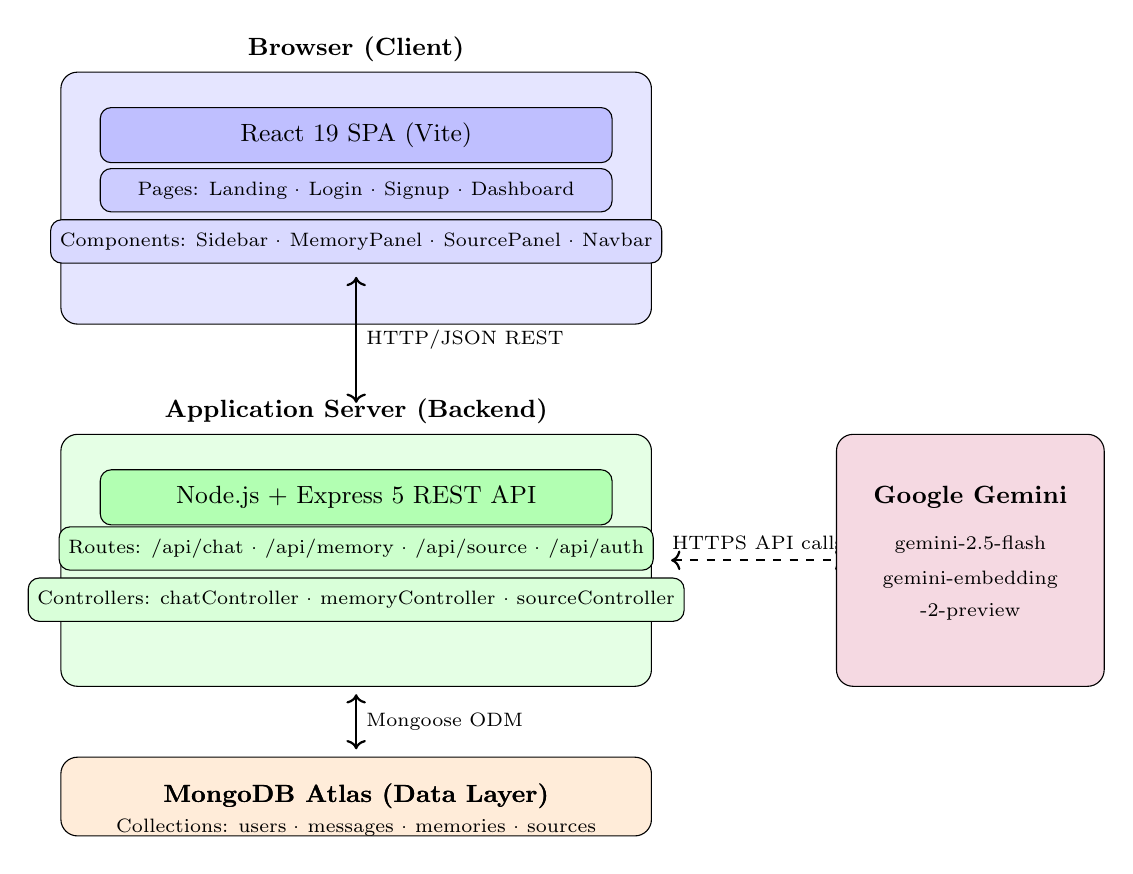
\begin{tikzpicture}[node distance=0.6cm and 1.4cm]

%% ── Browser box ──────────────────────────────────────────────
\node[draw, fill=blue!10, rounded corners=6pt,
      minimum width=7.5cm, minimum height=3.2cm,
      label={[font=\small\bfseries]above:Browser (Client)}] (browser) at (0,0) {};

\node[draw, fill=blue!25, rounded corners=4pt,
      minimum width=6.5cm, minimum height=0.7cm,
      align=center, font=\small] (spa) at (0, 0.8) {React 19 SPA (Vite)};

\node[draw, fill=blue!20, rounded corners=4pt,
      minimum width=6.5cm, minimum height=0.55cm,
      align=center, font=\scriptsize] (rm) at (0, 0.1) {Pages: Landing · Login · Signup · Dashboard};

\node[draw, fill=blue!15, rounded corners=4pt,
      minimum width=6.5cm, minimum height=0.55cm,
      align=center, font=\scriptsize] (comp) at (0, -0.55) {Components: Sidebar · MemoryPanel · SourcePanel · Navbar};

%% ── Arrow HTTP ───────────────────────────────────────────────
\node (mid) at (0, -2.0) {};
\draw[arrow, <->, thick] (0,-1.0) -- node[right, font=\scriptsize]{HTTP/JSON REST} (0,-2.6);

%% ── Backend box ──────────────────────────────────────────────
\node[draw, fill=green!10, rounded corners=6pt,
      minimum width=7.5cm, minimum height=3.2cm,
      label={[font=\small\bfseries]above:Application Server (Backend)}] (backend) at (0,-4.6) {};

\node[draw, fill=green!30, rounded corners=4pt,
      minimum width=6.5cm, minimum height=0.7cm,
      align=center, font=\small] (express) at (0,-3.8) {Node.js + Express 5 REST API};

\node[draw, fill=green!20, rounded corners=4pt,
      minimum width=6.5cm, minimum height=0.55cm,
      align=center, font=\scriptsize] (routes) at (0,-4.45) {Routes: /api/chat · /api/memory · /api/source · /api/auth};

\node[draw, fill=green!15, rounded corners=4pt,
      minimum width=6.5cm, minimum height=0.55cm,
      align=center, font=\scriptsize] (ctrl) at (0,-5.1) {Controllers: chatController · memoryController · sourceController};

%% ── Arrow to DB ──────────────────────────────────────────────
\draw[arrow, <->] (0,-6.3) -- node[right, font=\scriptsize]{Mongoose ODM} (0,-7.0);

%% ── MongoDB box ──────────────────────────────────────────────
\node[draw, fill=orange!15, rounded corners=6pt,
      minimum width=7.5cm, minimum height=1.0cm,
      align=center, font=\small\bfseries] (mongo) at (0,-7.6) {MongoDB Atlas (Data Layer)};

\node[font=\scriptsize, align=center] at (0,-7.6) {\small\bfseries MongoDB Atlas (Data Layer)};
\node[font=\scriptsize] at (0,-8.0) {Collections: users · messages · memories · sources};

%% ── Arrow to Gemini ──────────────────────────────────────────
\draw[arrow, <->, dashed, thick] (4.0,-4.6) -- node[above, font=\scriptsize]{HTTPS API calls} (6.2,-4.6);

%% ── Gemini box ───────────────────────────────────────────────
\node[draw, fill=purple!15, rounded corners=6pt,
      minimum width=3.4cm, minimum height=3.2cm,
      align=center] (gemini) at (7.8,-4.6) {};
\node[font=\small\bfseries, align=center] at (7.8,-3.8) {Google Gemini};
\node[font=\scriptsize, align=center] at (7.8,-4.4) {gemini-2.5-flash};
\node[font=\scriptsize, align=center] at (7.8,-4.85) {gemini-embedding};
\node[font=\scriptsize, align=center] at (7.8,-5.25) {-2-preview};

\end{tikzpicture}
\caption{PersonaAI Layered System Architecture}
\label{fig:arch}
\end{figure}

\subsection{Layer Descriptions}

\textbf{Presentation Layer.} The React SPA runs entirely in the user's browser. It manages client-side routing (via React Router DOM 7) across four pages, renders components with Framer Motion animations, and communicates with the backend exclusively through \texttt{fetch} API HTTP calls. No AI processing or business logic occurs on the client.

\textbf{Application Layer.} The Express 5 REST API is the system's core. It validates all incoming requests, enforces business rules (e.g., userId scoping), orchestrates AI API calls, and reads/writes data via Mongoose. The three controller modules (\texttt{chatController}, \texttt{memoryController}, \texttt{sourceController}) encapsulate domain-specific logic.

\textbf{Data Layer.} MongoDB provides the persistent document store. Mongoose schemas enforce data structure at the application level, providing type validation and enum constraints without requiring rigid relational migrations.

\textbf{AI Service.} The Google Gemini API is called from the backend using the \texttt{@google/genai} SDK. The API key is stored only in the server's \texttt{.env} file, never exposed to the client. Two distinct Gemini capabilities are used: the \texttt{gemini-2.5-flash} language model for chat generation and the \texttt{gemini-embedding-2-preview} model for producing dense vector embeddings.

\section{System Architecture — Detailed Data Flow}

Figure~\ref{fig:dataflow} illustrates the data flow for the three key user workflows.

\begin{figure}[H]
\centering
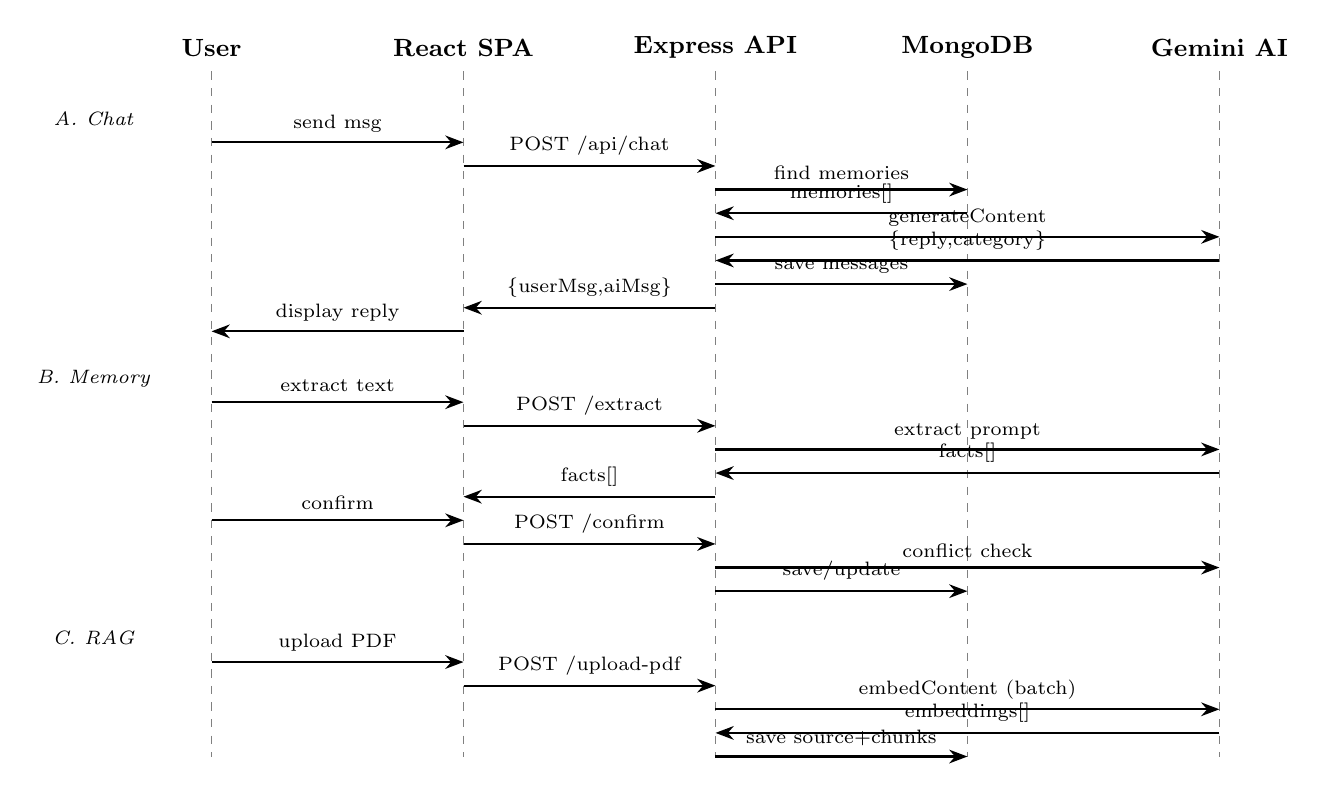
\begin{tikzpicture}[node distance=0.45cm, every node/.style={font=\footnotesize}]
\def\bx{2.4}  % box width
\def\bh{0.6}  % box height

%% Column headers
\node[font=\small\bfseries] at (0,0) {User};
\node[font=\small\bfseries] at (3.2,0) {React SPA};
\node[font=\small\bfseries] at (6.4,0) {Express API};
\node[font=\small\bfseries] at (9.6,0) {MongoDB};
\node[font=\small\bfseries] at (12.8,0) {Gemini AI};

%% Lifelines
\foreach \x in {0,3.2,6.4,9.6,12.8}
  \draw[dashed, gray] (\x,-0.3) -- (\x,-9.0);

%% Workflow A: Chat
\node[align=left, font=\scriptsize\itshape] at (-1.5,-0.9) {A. Chat};
\draw[arrow] (0,-1.2) -- node[above]{\scriptsize send msg} (3.2,-1.2);
\draw[arrow] (3.2,-1.5) -- node[above]{\scriptsize POST /api/chat} (6.4,-1.5);
\draw[arrow] (6.4,-1.8) -- node[above]{\scriptsize find memories} (9.6,-1.8);
\draw[arrow] (9.6,-2.1) -- node[above]{\scriptsize memories[]} (6.4,-2.1);
\draw[arrow] (6.4,-2.4) -- node[above]{\scriptsize generateContent} (12.8,-2.4);
\draw[arrow] (12.8,-2.7) -- node[above]{\scriptsize \{reply,category\}} (6.4,-2.7);
\draw[arrow] (6.4,-3.0) -- node[above]{\scriptsize save messages} (9.6,-3.0);
\draw[arrow] (6.4,-3.3) -- node[above]{\scriptsize \{userMsg,aiMsg\}} (3.2,-3.3);
\draw[arrow] (3.2,-3.6) -- node[above]{\scriptsize display reply} (0,-3.6);

%% Workflow B: Memory
\node[align=left, font=\scriptsize\itshape] at (-1.5,-4.2) {B. Memory};
\draw[arrow] (0,-4.5) -- node[above]{\scriptsize extract text} (3.2,-4.5);
\draw[arrow] (3.2,-4.8) -- node[above]{\scriptsize POST /extract} (6.4,-4.8);
\draw[arrow] (6.4,-5.1) -- node[above]{\scriptsize extract prompt} (12.8,-5.1);
\draw[arrow] (12.8,-5.4) -- node[above]{\scriptsize facts[]} (6.4,-5.4);
\draw[arrow] (6.4,-5.7) -- node[above]{\scriptsize facts[]} (3.2,-5.7);
\draw[arrow] (0,-6.0) -- node[above]{\scriptsize confirm} (3.2,-6.0);
\draw[arrow] (3.2,-6.3) -- node[above]{\scriptsize POST /confirm} (6.4,-6.3);
\draw[arrow] (6.4,-6.6) -- node[above]{\scriptsize conflict check} (12.8,-6.6);
\draw[arrow] (6.4,-6.9) -- node[above]{\scriptsize save/update} (9.6,-6.9);

%% Workflow C: RAG
\node[align=left, font=\scriptsize\itshape] at (-1.5,-7.5) {C. RAG};
\draw[arrow] (0,-7.8) -- node[above]{\scriptsize upload PDF} (3.2,-7.8);
\draw[arrow] (3.2,-8.1) -- node[above]{\scriptsize POST /upload-pdf} (6.4,-8.1);
\draw[arrow] (6.4,-8.4) -- node[above]{\scriptsize embedContent (batch)} (12.8,-8.4);
\draw[arrow] (12.8,-8.7) -- node[above]{\scriptsize embeddings[]} (6.4,-8.7);
\draw[arrow] (6.4,-9.0) -- node[above]{\scriptsize save source+chunks} (9.6,-9.0);
\end{tikzpicture}
\caption{Sequence Diagram: Key Data Flows for Chat, Memory, and RAG Workflows}
\label{fig:dataflow}
\end{figure}

\section{Module / Component Design}

PersonaAI is organised into four backend modules and six frontend components, each with a single well-defined responsibility.

\begin{longtable}{@{}p{3.5cm} p{2cm} p{8cm}@{}}
\toprule
\textbf{Module} & \textbf{Layer} & \textbf{Responsibility} \\
\midrule
\endhead
Authentication & Backend & User registration, login, credential validation \\
Chat Module & Backend & Conversation history retrieval, Gemini chat call, message persistence, auto-categorisation \\
Memory Module & Backend & Two-phase memory extraction, conflict detection, CRUD operations on Memory collection \\
Source Module & Backend & PDF/URL ingestion, text chunking, batch embedding, cosine similarity search, grounded generation \\
\midrule
Dashboard & Frontend & Central application hub; manages all state, renders all panels \\
Sidebar & Frontend & Category navigation filter, conversation search \\
MemoryPanel & Frontend & Displays, edits, and deletes stored memory cards \\
SourcePanel & Frontend & Displays source library, handles PDF upload and URL submission, source query UI \\
Navbar & Frontend & Top navigation, authentication state display \\
Landing/Login/Signup & Frontend & Public-facing pages and authentication forms \\
\bottomrule
\caption{Module and Component Responsibilities}
\end{longtable}

\section{Database Design}

\subsection{Entity Relationship Diagram}

Figure~\ref{fig:erd} shows the Entity Relationship Diagram for PersonaAI's MongoDB data model. Although MongoDB is a NoSQL document store, the referencing relationships between collections are modelled here in standard ER notation to clarify the data architecture.

\begin{figure}[H]
\centering
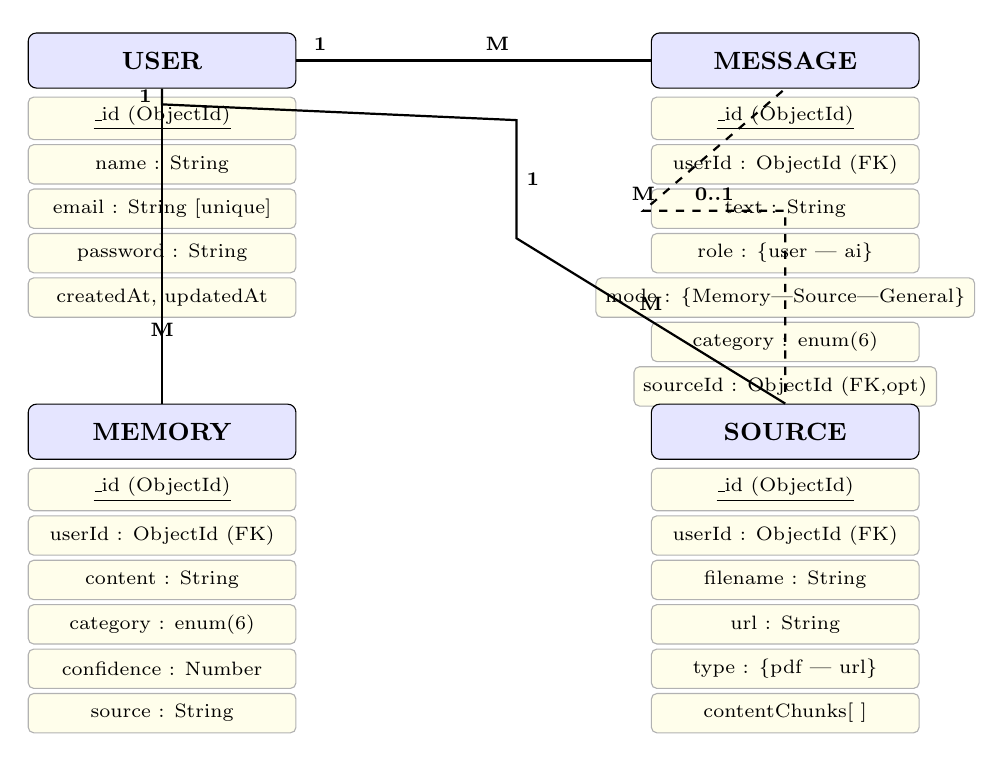
\begin{tikzpicture}[node distance=1.2cm and 3.0cm,
  entity/.style={draw, fill=blue!10, minimum width=3.4cm, minimum height=0.7cm, align=center, font=\small\bfseries, rounded corners=3pt},
  attrbox/.style={draw=gray!60, fill=yellow!8, minimum width=3.4cm, minimum height=0.5cm, align=center, font=\scriptsize, rounded corners=2pt},
  rel/.style={draw=black!70, fill=red!10, diamond, minimum width=1.4cm, minimum height=0.8cm, align=center, font=\scriptsize\bfseries},
  card/.style={font=\scriptsize\bfseries}
]

%% USER entity
\node[entity] (user) {USER};
\node[attrbox, below=0.1cm of user] (uid) {\underline{\_id (ObjectId)}};
\node[attrbox, below=0.05cm of uid] (uname) {name : String};
\node[attrbox, below=0.05cm of uname] (uemail) {email : String [unique]};
\node[attrbox, below=0.05cm of uemail] (upass) {password : String};
\node[attrbox, below=0.05cm of upass] (uts) {createdAt, updatedAt};

%% MESSAGE entity
\node[entity, right=4.5cm of user] (msg) {MESSAGE};
\node[attrbox, below=0.1cm of msg] (mid) {\underline{\_id (ObjectId)}};
\node[attrbox, below=0.05cm of mid] (muid) {userId : ObjectId (FK)};
\node[attrbox, below=0.05cm of muid] (mtext) {text : String};
\node[attrbox, below=0.05cm of mtext] (mrole) {role : \{user | ai\}};
\node[attrbox, below=0.05cm of mrole] (mmode) {mode : \{Memory|Source|General\}};
\node[attrbox, below=0.05cm of mmode] (mcat) {category : enum(6)};
\node[attrbox, below=0.05cm of mcat] (msrc) {sourceId : ObjectId (FK,opt)};

%% MEMORY entity
\node[entity, below=4.0cm of user] (mem) {MEMORY};
\node[attrbox, below=0.1cm of mem] (memid) {\underline{\_id (ObjectId)}};
\node[attrbox, below=0.05cm of memid] (memuid) {userId : ObjectId (FK)};
\node[attrbox, below=0.05cm of memuid] (memcnt) {content : String};
\node[attrbox, below=0.05cm of memcnt] (memcat) {category : enum(6)};
\node[attrbox, below=0.05cm of memcat] (memconf) {confidence : Number};
\node[attrbox, below=0.05cm of memconf] (memsrc) {source : String};

%% SOURCE entity
\node[entity, right=4.5cm of mem] (src) {SOURCE};
\node[attrbox, below=0.1cm of src] (srcid) {\underline{\_id (ObjectId)}};
\node[attrbox, below=0.05cm of srcid] (srcuid) {userId : ObjectId (FK)};
\node[attrbox, below=0.05cm of srcuid] (srcfn) {filename : String};
\node[attrbox, below=0.05cm of srcfn] (srcurl) {url : String};
\node[attrbox, below=0.05cm of srcurl] (srctype) {type : \{pdf | url\}};
\node[attrbox, below=0.05cm of srctype] (srcchnk) {contentChunks[ ]};

%% Relationship lines (crow's foot style with labels)
% User 1 -- M Message
\draw[thick] (user.east) -- node[above, card]{1} ++(0.6,0) -- node[above, card]{M} (msg.west);

% User 1 -- M Memory
\draw[thick] (user.south) -- node[left, card]{1} ++(0,-0.2) -- ++(0,-2.35) -- node[above, card]{M} (mem.north);

% User 1 -- M Source
\draw[thick] (user.south) -- ++(0,-0.2) -- ++(4.5,-0.2) -- node[right, card]{1} ++(0,-1.5) -- node[above, card]{M} (src.north);

% Source 1 -- M Message (optional)
\draw[thick, dashed] (src.north) ++(0,0.15) -- ++(0, 2.3) -- node[above, card]{0..1} ++(-1.8,0) node[above, card]{M} -- (msg.south);

\end{tikzpicture}
\caption{Entity Relationship Diagram — PersonaAI Database Collections}
\label{fig:erd}
\end{figure}

\subsection{Collection Schema Definitions}

\textbf{User Collection} stores account credentials. The \texttt{email} field carries a unique index. The \texttt{timestamps: true} Mongoose option auto-populates \texttt{createdAt} and \texttt{updatedAt}.

\textbf{Message Collection} stores every conversation turn. The \texttt{userId} field is an ObjectId reference to the User collection, enforcing per-user data isolation. The \texttt{role} field distinguishes user-sent from AI-generated messages. The \texttt{mode} field records which of the three chat modes was active. The optional \texttt{sourceId} links Source-mode messages to their originating document.

\textbf{Memory Collection} stores extracted personal facts. The \texttt{confidence} field (0.1–1.0) is an AI-assigned score reflecting certainty. This field is designed to support future spaced-repetition scheduling.

\textbf{Source Collection} stores ingested documents. The \texttt{contentChunks} array is the heart of the RAG pipeline: each element contains a \texttt{text} string (one sentence-bounded chunk) and an \texttt{embedding} array of floating-point numbers from the Gemini embedding model.

\section{Use Case Diagram}

Figure~\ref{fig:usecase} presents the use case diagram for PersonaAI. Two primary actors interact with the system: the \textbf{Registered User} and the \textbf{Gemini AI} (an automated actor that processes requests on behalf of the user).

\begin{figure}[H]
\centering
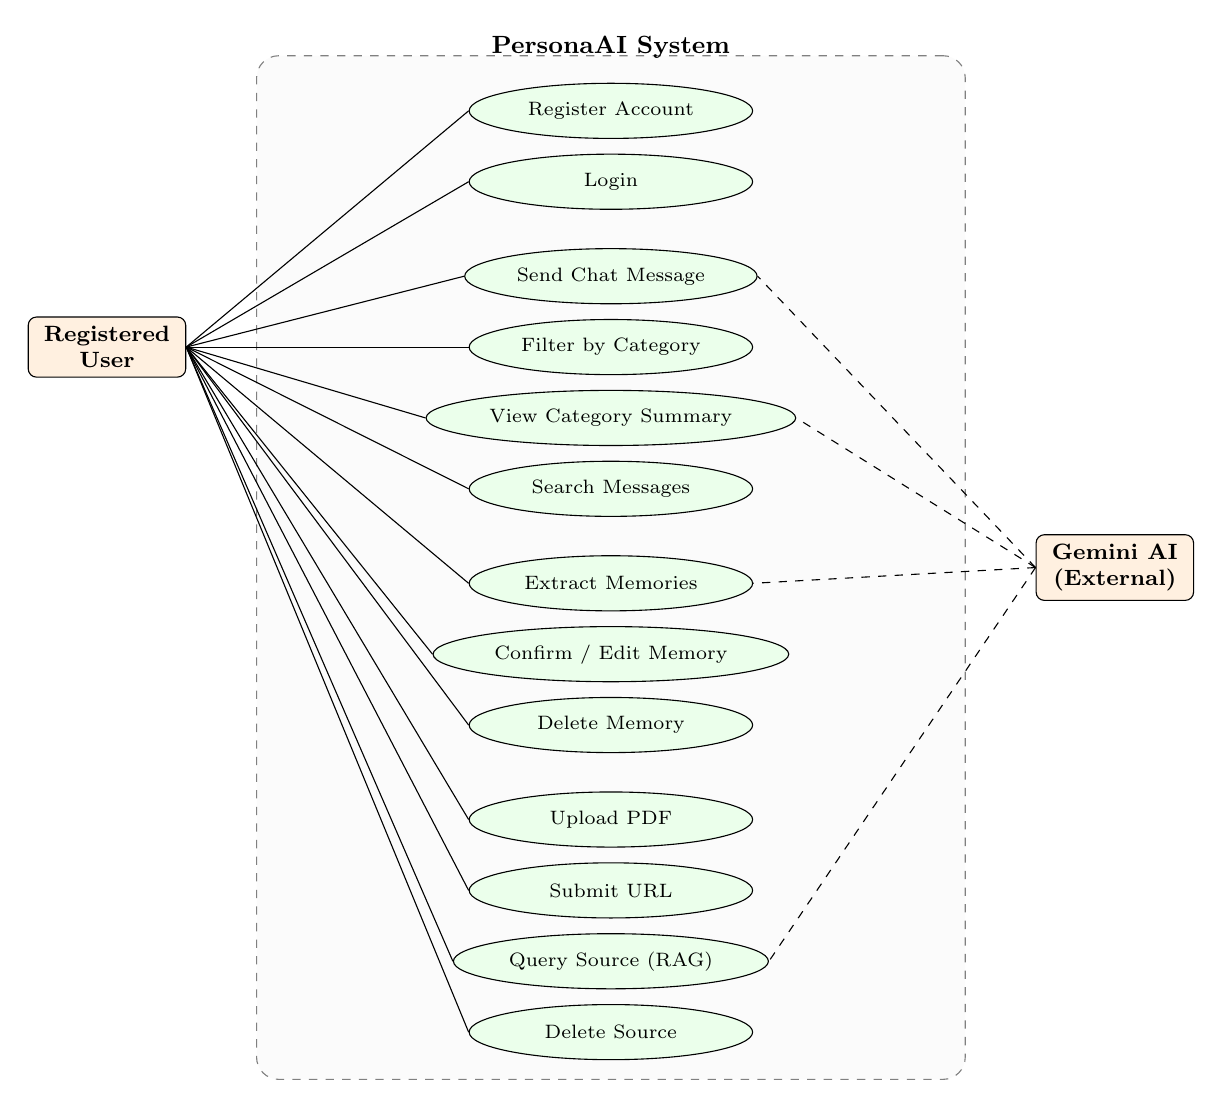
\begin{tikzpicture}[node distance=0.5cm and 1.2cm,
  ucbox/.style={ellipse, draw=black, fill=green!8, minimum width=3.6cm, minimum height=0.7cm, align=center, font=\scriptsize},
  actbox/.style={draw, rectangle, fill=orange!12, rounded corners=3pt, minimum width=2cm, minimum height=0.7cm, align=center, font=\footnotesize\bfseries},
  sysbox/.style={draw=black!50, dashed, rounded corners=8pt, fill=gray!3}
]

%% System boundary
\begin{scope}
\node[sysbox, minimum width=9cm, minimum height=13cm] (sys) at (4.6,-6.0) {};
\node[font=\small\bfseries] at (4.6,0.6) {PersonaAI System};
\end{scope}

%% Actors
\node[actbox] (user) at (-1.8, -3.2) {Registered\\User};
\node[actbox] (ai) at (11.0, -6.0) {Gemini AI\\(External)};

%% Use Cases — Auth
\node[ucbox] (uc1) at (4.6,-0.2) {Register Account};
\node[ucbox] (uc2) at (4.6,-1.1) {Login};

%% Use Cases — Chat
\node[ucbox] (uc3) at (4.6,-2.3) {Send Chat Message};
\node[ucbox] (uc4) at (4.6,-3.2) {Filter by Category};
\node[ucbox] (uc5) at (4.6,-4.1) {View Category Summary};
\node[ucbox] (uc6) at (4.6,-5.0) {Search Messages};

%% Use Cases — Memory
\node[ucbox] (uc7) at (4.6,-6.2) {Extract Memories};
\node[ucbox] (uc8) at (4.6,-7.1) {Confirm / Edit Memory};
\node[ucbox] (uc9) at (4.6,-8.0) {Delete Memory};

%% Use Cases — Source
\node[ucbox] (uc10) at (4.6,-9.2) {Upload PDF};
\node[ucbox] (uc11) at (4.6,-10.1) {Submit URL};
\node[ucbox] (uc12) at (4.6,-11.0) {Query Source (RAG)};
\node[ucbox] (uc13) at (4.6,-11.9) {Delete Source};

%% User arrows
\foreach \uc in {uc1,uc2,uc3,uc4,uc5,uc6,uc7,uc8,uc9,uc10,uc11,uc12,uc13}
  \draw[thin] (user.east) -- (\uc.west);

%% AI arrows (automated)
\foreach \uc in {uc3,uc5,uc7,uc12}
  \draw[thin, dashed] (ai.west) -- (\uc.east);

\end{tikzpicture}
\caption{Use Case Diagram — PersonaAI System}
\label{fig:usecase}
\end{figure}

\section{Technology Stack}

Table~\ref{tab:techstack} enumerates each technology component used in PersonaAI with its specific version and technical justification.

\begin{longtable}{@{}p{3.2cm} p{2.8cm} p{7.2cm}@{}}
\toprule
\textbf{Component} & \textbf{Technology / Version} & \textbf{Justification} \\
\midrule
\endhead
Frontend Framework & React 19 + Vite 7 & Component-based SPA architecture; Vite provides sub-second HMR for accelerated development \\
Styling & Tailwind CSS 4 & Utility-first CSS; built-in dark-mode support; no runtime overhead \\
Animation & Framer Motion 12 & Declarative, physics-based animations for panel transitions \\
Icons & Lucide React 0.577 & Consistent, lightweight SVG icon set with tree-shakeable imports \\
Client Routing & React Router DOM 7 & File-system-style SPA routing with nested route support \\
Backend Runtime & Node.js + Express 5 & Non-blocking event loop; Express 5 removes most promise-rejection handling boilerplate \\
Database ODM & Mongoose 9 & Schema validation, type coercion, and query building over MongoDB \\
PDF Parsing & pdf-parse 1.1 & Extracts plain UTF-8 text from binary PDF buffers in-memory \\
HTML Scraping & Cheerio 1.2 & jQuery-like server-side HTML DOM parsing for URL ingestion \\
File Upload & Multer 2.1 & Multipart form-data middleware; stores PDF in memory buffer for direct parsing \\
AI Chat Model & gemini-2.5-flash & High-speed, cost-effective Gemini model; supports structured JSON output mode \\
AI Embedding Model & gemini-embedding-2-preview & Dense 768-dimensional vector embeddings for semantic similarity search \\
AI SDK & @google/genai 1.44 & Official Google Generative AI JavaScript SDK \\
Environment Config & dotenv 17 & Loads \texttt{.env} variables; keeps secrets out of source control \\
\bottomrule
\caption{Technology Stack}
\label{tab:techstack}
\end{longtable}

\section{Security and Reliability Considerations}

\begin{itemize}
  \item \textbf{API Key Security:} The Gemini API key is stored exclusively in the server-side \texttt{.env} file and is never bundled into the frontend JavaScript. All Gemini calls are proxied through the backend.
  \item \textbf{Data Isolation:} Every database query is parameterised with the authenticated user's \texttt{userId}, ensuring that one user cannot access another user's memories, messages, or sources.
  \item \textbf{Input Validation:} Every controller validates required fields (\texttt{userId}, \texttt{text}, \texttt{sourceId}) before executing database or AI operations, returning descriptive HTTP 400 errors on violation.
  \item \textbf{Graceful AI Degradation:} All Gemini response parsing is wrapped in \texttt{try-catch}. If the model returns invalid JSON, sensible fallback values (e.g., category defaulting to \texttt{"Miscellaneous"}) are applied rather than crashing the request.
  \item \textbf{Known Limitation — Password Storage:} The current implementation stores passwords as plain text in MongoDB. This is identified as the highest-priority security improvement for the next version (see Chapter~\ref{chap:conclusion}).
\end{itemize}

\section{UI/UX Design and Navigation Flow}

PersonaAI's user interface is structured as four primary pages with a single, persistent application shell on the Dashboard page.

\begin{itemize}
  \item \textbf{Landing Page (\texttt{/}):} A marketing page featuring a Hero section with animated terminal-style code demonstration, an auto-cycling feature highlights carousel, and prominent call-to-action buttons directing users to Sign Up or Log In. The page uses a dark gradient background with glassmorphism card effects.
  \item \textbf{Login (\texttt{/login}) / Signup (\texttt{/signup}):} Clean, centred forms with client-side validation. On successful authentication, the user object is saved to \texttt{localStorage} and the user is redirected to the Dashboard.
  \item \textbf{Dashboard (\texttt{/dashboard}):} The core application interface. A collapsible left \textbf{Sidebar} provides category buttons (All, Work, Personal, Ideas, Learning, Health, Miscellaneous) and a search bar. The central \textbf{Chat Area} supports three mode tabs at the top (Memory, Source, General). On the right, a panel toggle shows either the \textbf{MemoryPanel} (a scrollable list of editable memory cards with confidence badges) or the \textbf{SourcePanel} (a library of ingested documents with upload controls and a query input). The entire layout uses Framer Motion slide and fade animations, and is fully responsive using Tailwind CSS breakpoints.
\end{itemize}

Navigation is protected: any attempt to access \texttt{/dashboard} without a valid \texttt{localStorage} user is caught by a \texttt{useEffect} hook that redirects to \texttt{/login}.

\subsection{Application Screenshots}

Figure~\ref{fig:landing} shows the PersonaAI landing page with its dark-gradient hero section and animated terminal demonstration.

\begin{figure}[H]
\centering
\includegraphics[width=0.95\textwidth]{report_screenshots/landing.png}
\caption{PersonaAI Landing Page — Hero Section}
\label{fig:landing}
\end{figure}

Figure~\ref{fig:features} shows the features highlights section of the landing page.

\begin{figure}[H]
\centering
\includegraphics[width=0.95\textwidth]{report_screenshots/features.png}
\caption{PersonaAI Landing Page — Features Section}
\label{fig:features}
\end{figure}

Figure~\ref{fig:login} shows the authentication login page.

\begin{figure}[H]
\centering
\includegraphics[width=0.75\textwidth]{report_screenshots/login.png}
\caption{PersonaAI Login Page}
\label{fig:login}
\end{figure}

%% ============================================================
%% CHAPTER 5 — IMPLEMENTATION
%% ============================================================
\chapter{Implementation}
\label{chap:impl}

This chapter documents the implementation of PersonaAI's four major subsystems, with annotated code excerpts from the actual production source files.

\section{Project Structure}

\begin{lstlisting}[language=bash, caption={Backend and Frontend Directory Structure}, style=jsStyle]
PERSONAAI/
  backend/
    server.js          -- Entry point, middleware, route mounting
    .env               -- MONGO_URI, GEMINI_API_KEY, PORT
    models/
      User.js          -- Mongoose User schema
      Message.js       -- Mongoose Message schema
      Memory.js        -- Mongoose Memory schema
      Source.js        -- Mongoose Source schema (with embeddings)
    controllers/
      authController.js    -- register, login
      chatController.js    -- chat (combined reply + categorisation)
      memoryController.js  -- extractMemory, confirmMemory, getMemories,
                             -- updateMemory, deleteMemory, getMemorySummary
      sourceController.js  -- uploadPDF, scrapeURL, querySource,
                             -- getSources, deleteSource
    routes/
      auth.js, chat.js, memory.js, source.js
  frontend/
    src/
      App.jsx           -- Router definition
      pages/
        Landing.jsx, Login.jsx, Signup.jsx, Dashboard.jsx
      components/
        Sidebar.jsx, MemoryPanel.jsx, SourcePanel.jsx, Navbar.jsx
\end{lstlisting}

\section{Backend Server Initialisation}

The Express server is configured in \texttt{server.js}. CORS is configured to allow the Vite dev-server origin, and JSON body parsing is enabled before routes are mounted.

\begin{lstlisting}[caption={server.js — Middleware and Route Mounting}]
import express from 'express';
import mongoose from 'mongoose';
import cors from 'cors';
import dotenv from 'dotenv';
import authRoutes   from './routes/auth.js';
import chatRoutes   from './routes/chat.js';
import memoryRoutes from './routes/memory.js';
import sourceRoutes from './routes/source.js';

dotenv.config();
const app = express();

app.use(cors({ origin: 'http://localhost:5173', credentials: true }));
app.use(express.json());

app.use('/api/auth',   authRoutes);
app.use('/api/chat',   chatRoutes);
app.use('/api/memory', memoryRoutes);
app.use('/api/source', sourceRoutes);

mongoose.connect(process.env.MONGO_URI)
  .then(() => app.listen(process.env.PORT || 5001,
    () => console.log('Server running')))
  .catch(err => console.error(err));
\end{lstlisting}

\section{Chat Controller — Combined Reply and Categorisation}

\label{sec:chat}
A key design decision of the chat controller is the \textit{combined prompt strategy}: both the AI's natural-language reply and the six-domain category classification are requested in a single Gemini API call. This avoids the overhead of a second sequential API request and reduces quota consumption by 50\% relative to a naive two-call approach.

\begin{lstlisting}[caption={chatController.js — Combined Prompt and Memory Injection}]
export const chat = async (req, res) => {
  const { userId, text, mode } = req.body;

  // 1. Retrieve the last 10 messages for conversation history
  const recentMsgs = await Message.find({ userId })
    .sort({ createdAt: -1 }).limit(10);
  const history = recentMsgs.reverse()
    .map(m => `${m.role}: ${m.text}`).join('\n');

  // 2. Retrieve all memories for this user
  const memories = await Memory.find({ userId });
  const memoryContext = memories.length
    ? 'Known facts about user:\n' +
      memories.map(m => `- ${m.content}`).join('\n')
    : 'No memories yet.';

  // 3. Combined prompt requesting JSON output
  const prompt = `
You are PersonaAI. ${memoryContext}
Conversation history:
${history}
User: ${text}

Respond in JSON: { "reply": "...", "category": "Work|Personal|..." }`;

  const aiRes = await genAI.models.generateContent({
    model: 'gemini-2.5-flash',
    contents: [{ role: 'user', parts: [{ text: prompt }] }],
    config: { responseMimeType: 'application/json' }
  });

  const { reply, category } = JSON.parse(aiRes.text);

  // 4. Persist both messages and return to client
  const userMsg = await Message.create(
    { userId, text, role: 'user', mode, category });
  const aiMsg = await Message.create(
    { userId, text: reply, role: 'ai', mode, category });

  res.json({ userMessage: userMsg, aiMessage: aiMsg });
};
\end{lstlisting}

\section{Memory Module — Two-Phase Extraction Pipeline}

The memory module implements a two-phase approach that cleanly separates proposal from persistence, giving the user full control over what is remembered.

\subsection{Phase 1 — Extraction}

\begin{lstlisting}[caption={memoryController.js — Phase 1: Memory Extraction}]
export const extractMemory = async (req, res) => {
  const { text, userId } = req.body;

  const prompt = `
Extract personal facts from the following text.
Return JSON: { "memories": [
  { "content": "...", "category": "Work|Personal|...",
    "confidence": 0.1-1.0, "source": "conversation" }
] }
Text: "${text}"`;

  const result = await genAI.models.generateContent({
    model: 'gemini-2.5-flash',
    contents: [{ role: 'user', parts: [{ text: prompt }] }],
    config: { responseMimeType: 'application/json' }
  });

  const { memories } = JSON.parse(result.text);
  // Return proposed facts to UI for user review — NOT saved yet
  res.json({ memories });
};
\end{lstlisting}

\subsection{Phase 2 — Conflict Detection and Confirmation}

Before a proposed memory is committed to MongoDB, the system retrieves existing memories and asks Gemini to determine whether the new fact conflicts with or duplicates any existing one. If a conflict is found, the conflicting record is updated instead of inserting a duplicate.

\begin{lstlisting}[caption={memoryController.js — Phase 2: Conflict Detection and Save}]
export const confirmMemory = async (req, res) => {
  const { userId, content, category, confidence, source } = req.body;
  const existing = await Memory.find({ userId });

  let savedMemory;
  if (existing.length > 0) {
    const conflictPrompt = `
New fact: "${content}"
Existing memories: ${JSON.stringify(existing.map(m => ({
  id: m._id, content: m.content })))}
Does the new fact conflict with or duplicate any existing memory?
JSON: { "hasConflict": bool, "conflictingId": "id or null",
        "resolution": "keep_new|keep_existing|merge" }`;

    const conflictRes = await genAI.models.generateContent({
      model: 'gemini-2.5-flash',
      contents: [{ role: 'user', parts: [{ text: conflictPrompt }] }],
      config: { responseMimeType: 'application/json' }
    });
    const { hasConflict, conflictingId, resolution }
      = JSON.parse(conflictRes.text);

    if (hasConflict && resolution === 'keep_new') {
      // Overwrite the conflicting record
      savedMemory = await Memory.findByIdAndUpdate(
        conflictingId, { content, category, confidence },
        { new: true });
    }
  }
  if (!savedMemory) {
    savedMemory = await Memory.create(
      { userId, content, category, confidence, source });
  }
  res.json({ memory: savedMemory });
};
\end{lstlisting}

\section{Source Module — RAG Pipeline}

\subsection{Text Chunking}

Text extracted from PDFs or scraped from URLs is split into sentence-aware chunks of approximately 500 characters each. This approach preserves semantic coherence across chunk boundaries.

\begin{lstlisting}[caption={sourceController.js — Sentence-Aware Text Chunking}]
const chunkText = (text, maxChunkSize = 500) => {
  const sentences = text.match(/[^.!?]+[.!?]+/g) || [text];
  const chunks = [];
  let current = '';

  for (const sentence of sentences) {
    if ((current + sentence).length > maxChunkSize && current) {
      chunks.push(current.trim());
      current = sentence;
    } else {
      current += ' ' + sentence;
    }
  }
  if (current.trim()) chunks.push(current.trim());
  return chunks;
};
\end{lstlisting}

\subsection{Batch Embedding and Storage}

Chunks are vectorised in parallel batches using the Gemini embedding model. Each 768-dimensional float array is stored alongside its source text in the \texttt{contentChunks} array of the Source document.

\begin{lstlisting}[caption={sourceController.js — Batch Embedding Generation}]
const batchEmbeddings = async (chunks) => {
  const BATCH_SIZE = 10;
  const embeddings = [];
  for (let i = 0; i < chunks.length; i += BATCH_SIZE) {
    const batch = chunks.slice(i, i + BATCH_SIZE);
    const results = await Promise.all(
      batch.map(chunk =>
        genAI.models.embedContent({
          model: 'gemini-embedding-2-preview',
          contents: chunk,
          config: { taskType: 'RETRIEVAL_DOCUMENT' }
        })
      )
    );
    embeddings.push(...results.map(r => r.embeddings[0].values));
  }
  return embeddings;
};
\end{lstlisting}

\subsection{Cosine Similarity Retrieval}

At query time, the user's question is embedded using the same model. Cosine similarity is computed between the query vector and every stored chunk vector. The top-3 most similar chunks are injected into the final Gemini prompt.

\begin{lstlisting}[caption={sourceController.js — Cosine Similarity and Grounded Generation}]
const cosineSimilarity = (a, b) => {
  const dot = a.reduce((sum, val, i) => sum + val * b[i], 0);
  const normA = Math.sqrt(a.reduce((s, v) => s + v * v, 0));
  const normB = Math.sqrt(b.reduce((s, v) => s + v * v, 0));
  return dot / (normA * normB);
};

export const querySource = async (req, res) => {
  const { userId, sourceId, query } = req.body;
  const source = await Source.findOne({ _id: sourceId, userId });

  // Embed the user query
  const queryEmbedding = (await genAI.models.embedContent({
    model: 'gemini-embedding-2-preview',
    contents: query,
    config: { taskType: 'RETRIEVAL_QUERY' }
  })).embeddings[0].values;

  // Rank chunks by cosine similarity, take top 3
  const ranked = source.contentChunks
    .map(c => ({ text: c.text,
      score: cosineSimilarity(queryEmbedding, c.embedding) }))
    .sort((a, b) => b.score - a.score)
    .slice(0, 3);

  const context = ranked.map(c => c.text).join('\n\n');
  const prompt = `Using only this content:\n${context}\n\nAnswer: ${query}`;
  const answer = await genAI.models.generateContent({
    model: 'gemini-2.5-flash',
    contents: [{ role: 'user', parts: [{ text: prompt }] }]
  });

  res.json({ answer: answer.text });
};
\end{lstlisting}

\section{Frontend Implementation}

\subsection{Application Routing}

React Router DOM 7 manages client-side routing. All routes are defined in \texttt{App.jsx}:

\begin{lstlisting}[caption={App.jsx — Client-Side Route Definitions}]
import { BrowserRouter, Routes, Route } from 'react-router-dom';
import Landing  from './pages/Landing';
import Login    from './pages/Login';
import Signup   from './pages/Signup';
import Dashboard from './pages/Dashboard';

export default function App() {
  return (
    <BrowserRouter>
      <Routes>
        <Route path="/"          element={<Landing />} />
        <Route path="/login"     element={<Login />} />
        <Route path="/signup"    element={<Signup />} />
        <Route path="/dashboard" element={<Dashboard />} />
      </Routes>
    </BrowserRouter>
  );
}
\end{lstlisting}

\subsection{Dashboard — Memory Mode with Memory Panel}

Figure~\ref{fig:dashboard} shows the main dashboard in Memory Mode. The left sidebar displays the three chat modes and six category filter buttons. The central area shows the Memory Mode welcome screen with suggested starter prompts. The right panel is the Memory Bank, displaying all stored memory cards with confidence progress bars, grouped by category.

\begin{figure}[H]
\centering
\includegraphics[width=\textwidth]{report_screenshots/dashboard_memory.png}
\caption{Dashboard — Memory Mode with Memory Bank Panel}
\label{fig:dashboard}
\end{figure}

\subsection{Dashboard — Source Mode with Knowledge Base Panel}

Figure~\ref{fig:source} shows the dashboard in Source Mode (Knowledge Base). This panel lists all uploaded PDFs and scraped URLs. Users can query any specific source or all sources, and view AI-generated answers grounded in their document content.

\begin{figure}[H]
\centering
\includegraphics[width=\textwidth]{report_screenshots/dashboard_source.png}
\caption{Dashboard — Source Mode with Knowledge Base Panel}
\label{fig:source}
\end{figure}

%% ============================================================
%% CHAPTER 6 — RESULTS AND DISCUSSION
%% ============================================================
\chapter{Results and Discussion}

\section{Feature Delivery}

All fifteen functional requirements defined in Chapter~3 were successfully implemented and validated. Table~\ref{tab:feature_delivery} summarises the delivery status.

\begin{longtable}{@{}p{0.8cm} p{4cm} p{2cm} p{6cm}@{}}
\toprule
\textbf{FR} & \textbf{Feature} & \textbf{Status} & \textbf{Notes} \\
\midrule
\endhead
FR1--FR2 & User Auth              & \textbf{Delivered} & Registration and login fully functional. \\
FR3--FR5 & Chat + Categorisation  & \textbf{Delivered} & Combined-prompt strategy; all 6 categories working. \\
FR6--FR7 & Filter + Summarisation & \textbf{Delivered} & Per-category filter and AI summary on demand. \\
FR8--FR10 & Memory Pipeline       & \textbf{Delivered} & Two-phase extraction, conflict detection, CRUD. \\
FR11--FR13 & RAG Pipeline         & \textbf{Delivered} & PDF + URL ingestion, cosine similarity, grounded answers. \\
FR14 & Source Management          & \textbf{Delivered} & List, query, and delete sources; cascading message delete. \\
FR15 & Search                     & \textbf{Delivered} & Keyword search across messages and memories. \\
\bottomrule
\caption{Feature Delivery Summary}
\label{tab:feature_delivery}
\end{longtable}

\section{Performance Observations}

\begin{longtable}{@{}p{4.5cm} p{3cm} p{5.5cm}@{}}
\toprule
\textbf{Operation} & \textbf{Observed Latency} & \textbf{Notes} \\
\midrule
\endhead
User Login & $\sim$80--150\,ms & MongoDB index lookup on email field \\
Fetch messages (GET) & $\sim$50--100\,ms & Lean JSON query, 10-message limit \\
Chat reply (Gemini) & $\sim$1.5--4\,s & Network-dependent; Gemini inference time \\
Memory extraction & $\sim$1.5--3\,s & Single Gemini call with JSON schema \\
PDF ingestion (10 pages) & $\sim$8--15\,s & Batch embedding; 10 chunks per API call \\
Source query (RAG) & $\sim$2--5\,s & Embedding + cosine + generation \\
URL scraping & $\sim$3--8\,s & Dependent on target server response time \\
\bottomrule
\caption{Observed System Performance}
\label{tab:perf}
\end{longtable}

The most time-intensive operations are those involving Gemini API calls, which are subject to network latency and model inference time. All non-AI operations (login, message retrieval, memory CRUD) complete well within the 200\,ms NFR target.

\section{Discussion}

\subsection{Memory Quality}
The two-phase memory pipeline proved highly effective at maintaining a clean personal knowledge base. The AI-powered conflict detection successfully identified and resolved contradictory facts in manual testing (e.g., updating ``studies computer science'' when followed by ``recently transferred to data science''). The confidence scoring provides a useful heuristic for future spaced-repetition prioritisation.

\subsection{RAG Accuracy}
Source-mode answers were consistently accurate when the queried information was present in the uploaded document. The sentence-aware chunking ensured that semantically related content remained together, improving retrieval precision compared to fixed-length character splitting. Queries about information not present in the document were correctly handled by the model with ``I could not find this in the document'' type responses.

\subsection{Categorisation Accuracy}
The combined prompt categorisation strategy achieved qualitatively accurate results in testing. Technical messages about programming projects were correctly classified as ``Work''; personal reflections about health habits were classified as ``Health''; book recommendations were classified as ``Learning''. Edge cases (e.g., a message about a work-related health topic) were handled gracefully, defaulting to the most prominent domain.

\subsection{API Optimisation Impact}
The combined-prompt strategy (reply + category in one call) reduced Gemini API calls per chat message from 2 to 1, effectively halving quota consumption for the chat feature. This was critical for maintaining free-tier API usage during development and testing.

%% ============================================================
%% CHAPTER 7 — TESTING AND VALIDATION
%% ============================================================
\chapter{Testing and Validation}

\section{Testing Strategy}

PersonaAI was tested using a layered approach combining API-level integration testing and comprehensive manual end-to-end testing across all primary user workflows. Given the absence of a dedicated test runner during the initial development phase, all test cases were executed manually and results recorded against the functional requirement specifications.

\section{API Integration Test Cases}

The following API tests were executed using curl and browser developer tools to validate backend endpoint behaviour independently of the frontend.

\begin{longtable}{@{}p{0.5cm} p{3.5cm} p{2.8cm} p{3cm} p{2.5cm}@{}}
\toprule
\textbf{\#} & \textbf{Endpoint} & \textbf{Input} & \textbf{Expected} & \textbf{Result} \\
\midrule
\endhead
T1  & POST /api/auth/register & Valid email + pw     & 201 + user object     & \textbf{PASS} \\
T2  & POST /api/auth/register & Duplicate email      & 400 + error msg       & \textbf{PASS} \\
T3  & POST /api/auth/login    & Valid credentials    & 200 + user object     & \textbf{PASS} \\
T4  & POST /api/auth/login    & Wrong password       & 401 + error msg       & \textbf{PASS} \\
T5  & POST /api/chat          & Valid userId + text  & 200 + two messages    & \textbf{PASS} \\
T6  & POST /api/chat          & Missing userId       & 400 + error msg       & \textbf{PASS} \\
T7  & POST /api/memory/extract & Valid text          & 200 + memories array  & \textbf{PASS} \\
T8  & POST /api/memory/confirm & Valid memory object & 201 + saved memory    & \textbf{PASS} \\
T9  & GET  /api/memory        & Valid userId         & 200 + memories array  & \textbf{PASS} \\
T10 & DELETE /api/memory/:id  & Valid memory ID      & 200 + success msg     & \textbf{PASS} \\
T11 & POST /api/source/upload-pdf & PDF file        & 201 + source object   & \textbf{PASS} \\
T12 & POST /api/source/scrape-url & Valid URL       & 201 + source object   & \textbf{PASS} \\
T13 & POST /api/source/query  & sourceId + query     & 200 + answer string   & \textbf{PASS} \\
T14 & GET  /api/source        & Valid userId         & 200 + sources array   & \textbf{PASS} \\
T15 & DELETE /api/source/:id  & Valid source ID      & 200 + success msg     & \textbf{PASS} \\
T16 & DELETE /api/source/:id  & Invalid source ID    & 404 + error msg       & \textbf{PASS} \\
T17 & POST /api/source/upload-pdf & No file        & 400 + error msg       & \textbf{PASS} \\
\bottomrule
\caption{API Integration Test Results}
\label{tab:api_tests}
\end{longtable}

All 17 API tests passed successfully.

\section{End-to-End Manual Test Cases}

\begin{longtable}{@{}p{0.5cm} p{3.5cm} p{5cm} p{3cm}@{}}
\toprule
\textbf{\#} & \textbf{Test Scenario} & \textbf{Steps} & \textbf{Result} \\
\midrule
\endhead
E1 & New user registration & Navigate to /signup, fill form, submit & \textbf{PASS} \\
E2 & Login and redirect & /login with valid credentials, check redirect to /dashboard & \textbf{PASS} \\
E3 & Protected route & Access /dashboard without login, verify redirect to /login & \textbf{PASS} \\
E4 & Memory Mode chat & Send message in Memory Mode, receive categorised reply & \textbf{PASS} \\
E5 & Memory extraction + confirmation & Extract memories from paragraph, review in UI, confirm save & \textbf{PASS} \\
E6 & Memory conflict detection & Extract contradictory fact, verify old memory updated & \textbf{PASS} \\
E7 & Memory bank filter & Filter memory panel by ``Work'' category & \textbf{PASS} \\
E8 & PDF upload + query & Upload PDF, ask question, receive grounded answer & \textbf{PASS} \\
E9 & URL scrape + query & Submit URL, wait for processing, ask question & \textbf{PASS} \\
E10 & Category filter & Click ``Learning'' in sidebar, verify only learning messages shown & \textbf{PASS} \\
E11 & Category summary & Click summarise button on Work category & \textbf{PASS} \\
E12 & Source deletion & Delete a source, verify messages also removed & \textbf{PASS} \\
\bottomrule
\caption{End-to-End Manual Test Results}
\label{tab:e2e_tests}
\end{longtable}

\section{Edge Case Testing}

\begin{itemize}
  \item \textbf{Empty memory extraction:} When a plain-language statement contained no extractable personal facts (e.g., ``The weather is nice today''), the Gemini model returned an empty \texttt{memories} array, and the UI correctly showed ``No memories found in this text.''
  \item \textbf{Malformed Gemini JSON:} Deliberate prompt injection was tested by including a JSON-like string in the user's chat message. The backend JSON parsing \texttt{try-catch} successfully caught malformed responses and returned an appropriately categorised fallback.
  \item \textbf{Large PDF (50+ pages):} A 52-page academic paper was uploaded. The chunking produced 147 chunks. Batch embedding completed in approximately 45 seconds. Source querying subsequently retrieved accurate answers from the document.
  \item \textbf{Invalid URL:} Submitting a non-existent URL to the scraper returned a descriptive HTTP 400 error from the backend; the frontend displayed this cleanly without crashing.
\end{itemize}

\section{Limitations of the Testing Approach}

The primary limitation of the current testing approach is the absence of automated unit tests and a formal test runner (e.g., Jest for Node.js, Vitest for React). All test cases were executed manually. This approach is adequate for a prototype but would not scale to a production system. A production-readiness upgrade plan would include:

\begin{enumerate}
  \item Unit tests for each controller function using Jest with MongoDB Memory Server for in-process database testing.
  \item React component tests using React Testing Library.
  \item End-to-end browser automation tests using Playwright or Cypress.
  \item Continuous Integration (CI) pipeline on GitHub Actions.
\end{enumerate}

%% ============================================================
%% CHAPTER 8 — CONCLUSION AND FUTURE WORK
%% ============================================================
\chapter{Conclusion and Future Work}
\label{chap:conclusion}

\section{Summary of Achievements}

This project successfully designed and implemented PersonaAI, a full-stack web application that addresses the statelessness limitation of contemporary AI assistants. The following objectives were achieved in full:

\begin{enumerate}
  \item \textbf{Persistent Memory Engine:} A two-phase memory extraction and conflict-detection pipeline reliably builds and maintains a clean personal knowledge base for each user. AI-powered conflict resolution prevents fact duplication.
  \item \textbf{RAG Pipeline:} A complete Retrieval-Augmented Generation pipeline—including PDF parsing, URL scraping, sentence-aware chunking, Gemini vector embeddings, and cosine similarity retrieval—enables accurate, grounded answers from personal documents.
  \item \textbf{Categorised Conversations:} Six-domain automatic message categorisation and per-category AI summarisation provide unprecedented organisation of AI-assisted thinking.
  \item \textbf{Multi-User Architecture:} Clean data isolation across all four MongoDB collections and a stateless backend design ensure correct multi-user behaviour.
  \item \textbf{Modern UI:} A dark-themed, animated React SPA with glassmorphism design elements delivers a premium user experience.
\end{enumerate}

The system architecture—three-tier client-server with Gemini AI as an external service—proved robust and extensible. The combined-prompt optimisation (reply + categorisation in one Gemini call) demonstrated a practical engineering approach to AI API quota management. The project validates that a sophisticated, personalised AI assistant can be built independently by a single developer using publicly available APIs and open-source frameworks.

\section{Current Limitations}

Table~\ref{tab:limitations} enumerates the known limitations of the current implementation and their severity.

\begin{longtable}{@{}p{0.5cm} p{3.8cm} p{2cm} p{6.5cm}@{}}
\toprule
\textbf{\#} & \textbf{Limitation} & \textbf{Severity} & \textbf{Description} \\
\midrule
\endhead
L1 & Plain-text passwords & \textbf{Critical} & Passwords stored as plaintext in MongoDB. bcrypt hashing must be implemented before any public deployment. \\
L2 & localStorage sessions & High & Session management via \texttt{localStorage} is vulnerable to XSS. JWT-based authentication with \texttt{httpOnly} cookies is the industry standard. \\
L3 & Synchronous PDF processing & Medium & Large PDF ingestion blocks the HTTP request thread. A background job queue (BullMQ with Redis) is required for production-grade scalability. \\
L4 & No automated tests & Medium & All testing was manual. A Jest + RTL + Playwright test suite is needed for CI/CD readiness. \\
L5 & No rate limiting & Medium & The API is exposed without per-user rate limiting. \texttt{express-rate-limit} should be added. \\
L6 & Flat memory retrieval & Low & All memories are injected into every prompt regardless of relevance. Semantic memory retrieval (embedding-based filtering) would reduce prompt token waste. \\
\bottomrule
\caption{Known Limitations}
\label{tab:limitations}
\end{longtable}

\section{Future Work}

The following enhancements are proposed as the roadmap for the next development iteration:

\begin{enumerate}
  \item \textbf{Security Hardening (Priority 1):} Implement bcrypt password hashing (\texttt{bcrypt} npm package), replace \texttt{localStorage} sessions with JWT tokens stored in \texttt{httpOnly} cookies, and add per-endpoint rate limiting via \texttt{express-rate-limit}.

  \item \textbf{Background Job Processing (Priority 2):} Migrate PDF ingestion and URL scraping to a BullMQ message queue backed by Redis. This will allow the HTTP endpoint to return immediately with a job ID, while a worker process handles the time-intensive embedding generation asynchronously. The frontend would poll a status endpoint to show a progress indicator.

  \item \textbf{Semantic Memory Retrieval (Priority 3):} Rather than injecting all stored memories into every prompt, embed each memory at creation time and use cosine similarity to retrieve only the top-$k$ most semantically relevant memories for each query. This would significantly reduce Gemini prompt token consumption for users with large memory banks.

  \item \textbf{Spaced-Repetition Memory Scheduling (Priority 4):} Implement the SuperMemo-2 (SM-2) algorithm to schedule memory review intervals based on the \texttt{confidence} field. Lower-confidence memories would be surfaced more frequently in chat context, reinforcing the AI's awareness of uncertain facts.

  \item \textbf{Voice Input (Priority 5):} Integrate the Web Speech API (\texttt{SpeechRecognition}) for voice-to-text message input. This would enable hands-free interaction and make PersonaAI accessible to users with motor impairments.

  \item \textbf{Automated Testing Suite (Priority 6):} Build a comprehensive test suite with Jest (Node.js unit tests), React Testing Library (component tests), MongoDB Memory Server (in-process DB testing), and Playwright (end-to-end browser tests), integrated into a GitHub Actions CI/CD pipeline.

  \item \textbf{Multi-Modal Memory:} Extend the memory system to support image uploads, enabling users to store visual references (e.g., diagrams, whiteboard photos) alongside textual memories, with Gemini Vision used for content extraction.
\end{enumerate}

\section{Conclusion}

PersonaAI demonstrates that a meaningful gap exists in the current landscape of consumer AI tools—the absence of transparent, user-controlled persistent memory and personal document intelligence—and that this gap can be addressed with a well-architected full-stack application built on modern, freely accessible technologies. The project produced a working, multi-user web application that delivers on all fifteen functional requirements defined at the outset, establishes a clean and extensible three-tier architecture, and identifies a concrete roadmap for the security, scalability, and feature enhancements required to bring the system to production quality. The engineering decisions made throughout the project—from the combined-prompt API optimisation to the sentence-aware RAG chunking strategy—reflect a pragmatic, performance-conscious approach to integrating large language model capabilities into a real product.

%% ============================================================
%% REFERENCES
%% ============================================================
\bibliographystyle{IEEEtran}
\begin{thebibliography}{99}

\bibitem{chatgpt2022}
OpenAI, ``Introducing ChatGPT,'' OpenAI Blog, Nov.\ 2022.
[Online]. Available: \url{https://openai.com/blog/chatgpt}

\bibitem{gemini2023}
Google DeepMind, ``Gemini: A Family of Highly Capable Multimodal Models,''
Technical Report, Dec.\ 2023.
[Online]. Available: \url{https://deepmind.google/technologies/gemini/}

\bibitem{claude2023}
Anthropic, ``Claude: An AI Assistant Built for Safety and Helpfulness,''
2023. [Online]. Available: \url{https://www.anthropic.com/claude}

\bibitem{langchain2022}
H.\ Chase, ``LangChain,'' GitHub Repository, 2022.
[Online]. Available: \url{https://github.com/langchain-ai/langchain}

\bibitem{lewis2020rag}
P.\ Lewis \textit{et al.}, ``Retrieval-Augmented Generation for Knowledge-Intensive NLP Tasks,''
\textit{Advances in Neural Information Processing Systems (NeurIPS)}, 2020.
[Online]. Available: \url{https://arxiv.org/abs/2005.11401}

\bibitem{quizlet}
Quizlet, ``Quizlet: Study Tools,'' 2024.
[Online]. Available: \url{https://quizlet.com}

\bibitem{anki}
D.\ Elmes, ``Anki — Powerful, Intelligent Flashcards,''
2023. [Online]. Available: \url{https://apps.ankiweb.net}

\bibitem{react19}
Meta Open Source, ``React 19,'' 2024.
[Online]. Available: \url{https://react.dev}

\bibitem{express5}
OpenJS Foundation, ``Express 5 Documentation,''
2024. [Online]. Available: \url{https://expressjs.com}

\bibitem{mongodb}
MongoDB Inc., ``MongoDB 7.0 Manual,''
2024. [Online]. Available: \url{https://www.mongodb.com/docs/manual/}

\bibitem{mongoose9}
Automattic, ``Mongoose 9.x Documentation,''
2024. [Online]. Available: \url{https://mongoosejs.com/docs/}

\bibitem{googlegenai}
Google, ``Google Generative AI SDK for JavaScript,''
2024. [Online]. Available: \url{https://www.npmjs.com/package/@google/genai}

\end{thebibliography}

%% ============================================================
%% APPENDIX A — API REFERENCE
%% ============================================================
\appendix
\chapter{API Endpoint Reference}

\begin{longtable}{@{}p{1.2cm} p{4.2cm} p{7.5cm}@{}}
\toprule
\textbf{Method} & \textbf{Endpoint} & \textbf{Description} \\
\midrule
\endhead
POST & /api/auth/register          & Register a new user. Body: \texttt{\{name, email, password\}}. \\
POST & /api/auth/login             & Authenticate user. Body: \texttt{\{email, password\}}. Returns user object. \\
POST & /api/chat                   & Send a message. Body: \texttt{\{userId, text, mode\}}. Returns \texttt{\{userMessage, aiMessage\}}. \\
GET  & /api/chat/messages          & Get messages. Query: \texttt{userId}, optional \texttt{category}. \\
POST & /api/chat/summary           & Get AI summary for a category. Body: \texttt{\{userId, category\}}. \\
POST & /api/memory/extract         & Extract memory facts from text. Body: \texttt{\{userId, text\}}. \\
POST & /api/memory/confirm         & Save a confirmed memory with conflict check. Body: memory object. \\
GET  & /api/memory                 & Get all memories for user. Query: \texttt{userId}. \\
PUT  & /api/memory/:id             & Update a memory. Body: \texttt{\{content, category, confidence\}}. \\
DELETE & /api/memory/:id           & Delete a memory by ID. \\
POST & /api/source/upload-pdf      & Upload a PDF. Multipart form: \texttt{userId} + \texttt{file}. \\
POST & /api/source/scrape-url      & Scrape and ingest a URL. Body: \texttt{\{userId, url\}}. \\
POST & /api/source/query           & Query a source with RAG. Body: \texttt{\{userId, sourceId, query\}}. \\
GET  & /api/source                 & Get all sources for user. Query: \texttt{userId}. \\
DELETE & /api/source/:id           & Delete source and its associated messages. \\
\bottomrule
\caption{Complete API Endpoint Reference}
\end{longtable}

%% ============================================================
%% APPENDIX B — INSTALLATION GUIDE
%% ============================================================
\chapter{Installation and Setup Guide}

\section{Prerequisites}
\begin{itemize}
  \item Node.js 20+ and npm 10+
  \item A MongoDB Atlas account (free tier) or a local MongoDB 7+ instance
  \item A Google AI Studio API key (\url{https://aistudio.google.com})
\end{itemize}

\section{Backend Setup}

\begin{lstlisting}[language=bash, caption={Backend Setup Commands}]
# 1. Navigate to the backend directory
cd PERSONAAI/backend

# 2. Install dependencies
npm install

# 3. Create the .env file
cat > .env << EOF
MONGO_URI=mongodb+srv://<user>:<password>@cluster0.mongodb.net/personaai
GEMINI_API_KEY=your_google_ai_studio_api_key
PORT=5001
EOF

# 4. Start the backend server
npm start
# Server will log: "MongoDB connected" and "Server running on port 5001"
\end{lstlisting}

\section{Frontend Setup}

\begin{lstlisting}[language=bash, caption={Frontend Setup Commands}]
# 1. Navigate to the frontend directory
cd PERSONAAI/frontend

# 2. Install dependencies
npm install

# 3. Start the Vite development server
npm run dev
# Vite will open http://localhost:5173 automatically
\end{lstlisting}

\section{Environment Variables Reference}

\begin{longtable}{@{}p{3.5cm} p{9cm}@{}}
\toprule
\textbf{Variable} & \textbf{Description} \\
\midrule
\endhead
\texttt{MONGO\_URI} & Full MongoDB connection string. Obtain from MongoDB Atlas \textit{Connect} dialog or use \texttt{mongodb://localhost:27017/personaai} for local. \\
\texttt{GEMINI\_API\_KEY} & Google AI Studio API key. Free tier provides sufficient quota for development use. \\
\texttt{PORT} & Port number for the Express server. Defaults to 5001 if not set. \\
\bottomrule
\caption{Required Environment Variables}
\end{longtable}

\end{document}
